% questions.tex —— 2004 年·北京卷·文科 · 题目内容片段（无答案）
% 由 tools/generate_projects.py 依来源总账自 2004/2004_数学真题_北京文_试题.md 生成，勿手改（改源 MD 后重跑）


\begin{gktip}
\textbf{来源说明}：本题面依据固定源 PDF 两页 A3 题面逐题转录，原卷印刷页码 158–159。固定源不附答案，答案和解析均由本库独立复算。

\textbf{图形说明}：第 6、16、17 题的原卷图形重绘为 TikZ 矢量图。图形标记所指的 PNG 不随仓库保存。
\end{gktip}

\gkpart{一、选择题（本大题共 8 小题，每小题 5 分，共 40 分．在每小题给出的四个选项中，只有一项是符合题目要求的）}

\begin{question}
\gkti{1}设 $M=\{x\mid -2\le x\le 2\}$，$N=\{x\mid x<1\}$，则 $M\cap N$ 等于\mbox{（　　）}

（A）$\{x\mid 1<x<2\}$　　（B）$\{x\mid -2<x<1\}$

（C）$\{x\mid 1<x\le 2\}$　　（D）$\{x\mid -2\le x<1\}$

\end{question}
\begin{question}
\gkti{2}满足条件 $|z|=|3+4\mathrm{i}|$ 的复数 $z$ 在复平面上对应点的轨迹是\mbox{（　　）}

（A）一条直线　　（B）两条直线　　（C）圆　　（D）椭圆

\end{question}
\begin{question}
\gkti{3}设 $m, n$ 是两条不同的直线，$\alpha, \beta, \gamma$ 是三个不同的平面，给出下列四个命题：

① 若 $m\perp\alpha$，$n\parallel\alpha$，则 $m\perp n$；

② 若 $\alpha\parallel\beta$，$\beta\parallel\gamma$，$m\perp\alpha$，则 $m\perp\gamma$；

③ 若 $m\parallel\alpha$，$n\parallel\alpha$，则 $m\parallel n$；

④ 若 $\alpha\perp\gamma$，$\beta\perp\gamma$，则 $\alpha\parallel\beta$．

其中正确命题的序号是\mbox{（　　）}

（A）①和②　　（B）②和③　　（C）③和④　　（D）①和④

\end{question}
\begin{question}
\gkti{4}已知 $a, b, c$ 满足 $c<b<a$ 且 $ac<0$，那么下列选项中一定成立的是\mbox{（　　）}

（A）$ab>ac$　　（B）$c(b-a)<0$　　（C）$cb^2<ab^2$　　（D）$ac(a-c)>0$

\end{question}
\begin{question}
\gkti{5}从长度分别为 $1, 2, 3, 4, 5$ 的五条线段中，任取三条的不同取法共有 $n$ 种．在这些取法中，以取出的三条线段为边可组成的钝角三角形的个数为 $m$，则 $\dfrac{m}{n}$ 等于\mbox{（　　）}

（A）$\dfrac{1}{10}$　　（B）$\dfrac{1}{5}$　　（C）$\dfrac{3}{10}$　　（D）$\dfrac{2}{5}$

\Needspace{0.4\textheight}
\end{question}
\begin{question}
\gkti{6}如图，在正方体 $ABCD-A_1B_1C_1D_1$ 中，$P$ 是侧面 $BB_1C_1C$ 内一动点，若 $P$ 到直线 $BC$ 与直线 $C_1D_1$ 的距离相等，则动点 $P$ 的轨迹所在的曲线是\mbox{（　　）}
\nopagebreak[4]
\begin{center}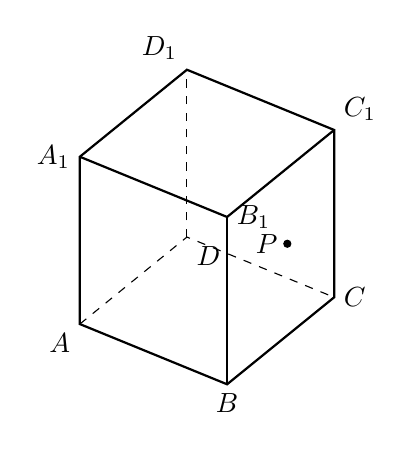
\begin{tikzpicture}[>=stealth, scale=0.85]
  % 顶点坐标
  \coordinate (A) at (0, 0);
  \coordinate (B) at (2.2, -0.9);
  \coordinate (C) at (3.8, 0.4);
  \coordinate (D) at (1.6, 1.3);
  \coordinate (A1) at (0, 2.5);
  \coordinate (B1) at (2.2, 1.6);
  \coordinate (C1) at (3.8, 2.9);
  \coordinate (D1) at (1.6, 3.8);

  % 侧面 BB1C1C 内动点 P
  \coordinate (P) at (3.1, 1.2);

  % 虚线（不可见棱）
  \draw[dashed, thin] (A) -- (D) -- (C);
  \draw[dashed, thin] (D) -- (D1);

  % 实线（可见棱）
  \draw[thick] (A) -- (B) -- (C) -- (C1) -- (D1) -- (A1) -- cycle;
  \draw[thick] (B) -- (B1);
  \draw[thick] (A1) -- (B1) -- (C1);

  % 动点 P 及其标注
  \filldraw[black] (P) circle (1.5pt);
  \node[left] at (P) {$P$};

  % 顶点标签
  \node[below left] at (A) {$A$};
  \node[below] at (B) {$B$};
  \node[right] at (C) {$C$};
  \node[below right] at (D) {$D$};
  \node[left] at (A1) {$A_1$};
  \node[right] at (B1) {$B_1$};
  \node[above right] at (C1) {$C_1$};
  \node[above left] at (D1) {$D_1$};
\end{tikzpicture}
\end{center}
\nopagebreak[4]
（A）直线　　（B）圆　　（C）双曲线　　（D）抛物线

\end{question}
\begin{question}
\gkti{7}函数 $f(x)=x^2-2ax-3$ 在区间 $[1, 2]$ 上存在反函数的充分必要条件是\mbox{（　　）}

（A）$a\in(-\infty, 1]$　　（B）$a\in[2, +\infty)$

（C）$a\in(-\infty, 1]\cup[2, +\infty)$　　（D）$a\in[1, 2]$

\end{question}
\begin{question}
\gkti{8}函数 $f(x)=\begin{cases} x, & x\in P, \\ -x, & x\in M, \end{cases}$ 其中 $P, M$ 为实数集 $\mathbf{R}$ 的两个非空子集，又规定 $f(P)=\{y\mid y=f(x), x\in P\}$，$f(M)=\{y\mid y=f(x), x\in M\}$，给出下列四个判断：

① 若 $P\cap M=\emptyset$，则 $f(P)\cup f(M)=\emptyset$；

② 若 $P\cap M\neq\emptyset$，则 $f(P)\cap f(M)\neq\emptyset$；

③ 若 $P\cup M=\mathbf{R}$，则 $f(P)\cup f(M)=\mathbf{R}$；

④ 若 $P\cup M\neq\mathbf{R}$，则 $f(P)\cup f(M)\neq\mathbf{R}$．

其中正确判断有\mbox{（　　）}

（A）$3$ 个　　（B）$2$ 个　　（C）$1$ 个　　（D）$0$ 个

\end{question}
\gkpart{二、填空题（本大题共 6 小题，每小题 5 分，共 30 分．把答案填在题中横线上）}

\begin{question}
\gkti{9}函数 $y=\sin x\cos x$ 的最小正周期是 \underline{\hspace{3em}}．

\end{question}
\begin{question}
\gkti{10}方程 $\lg(x^2+2)=\lg x+\lg 3$ 的解是 \underline{\hspace{3em}}．

\end{question}
\begin{question}
\gkti{11}某地球仪上北纬 $30^\circ$ 纬线的长度为 $12\pi\text{ cm}$，该地球仪的半径是 \underline{\hspace{3em}}$\text{ cm}$，表面积是 \underline{\hspace{3em}}$\text{ cm}^2$．

\end{question}
\begin{question}
\gkti{12}圆 $x^2+(y+1)^2=1$ 的圆心坐标是 \underline{\hspace{3em}}，如果直线 $x+y+a=0$ 与该圆有公共点，那么实数 $a$ 的取值范围是 \underline{\hspace{3em}}．

\end{question}
\begin{question}
\gkti{13}在函数 $f(x)=ax^2+bx+c$ 中，若 $a, b, c$ 成等比数列且 $f(0)=-4$，则 $f(x)$ 有最 \underline{\hspace{2em}} 值（填“大”或“小”），且该值为 \underline{\hspace{3em}}．

\end{question}
\begin{question}
\gkti{14}定义“等和数列”：在一个数列中，如果每一项与它的后一项的和都为同一个常数，那么这个数列叫做等和数列，这个常数叫做该数列的公和．已知数列 $\{a_n\}$ 是等和数列，且 $a_1=2$，公和为 $5$，那么 $a_{18}$ 的值为 \underline{\hspace{3em}}，且这个数列的前 $21$ 项和 $S_{21}$ 的计算公式为 \underline{\hspace{3em}}．

\end{question}
\gkpart{三、解答题（本大题共 6 小题，共 80 分．解答应写出文字说明、证明过程或演算步骤）}

\begin{question}
\gkti{15}\textbf{（本小题满分 12 分）} 
在 $\triangle ABC$ 中，$\sin A+\cos A=\dfrac{\sqrt{2}}{2}$，$AC=2$，$AB=3$，求 $\tan A$ 的值和 $\triangle ABC$ 的面积．

\Needspace{0.4\textheight}
\end{question}
\begin{question}
\gkti{16}\textbf{（本小题满分 14 分）} 
如图，在正三棱柱 $ABC-A_1B_1C_1$ 中，$AB=2$，$AA_1=2$，由顶点 $B$ 沿棱柱侧面经过棱 $AA_1$ 到顶点 $C$ 的最短路线与 $AA_1$ 的交点为 $M$，求：

（1）该三棱柱的侧面展开图的对角线长；

（2）该最短路线的长与 $\dfrac{A_1M}{AM}$ 的值；

（3）平面 $C_1MB$ 与平面 $ABC$ 所成二面角（锐角）的大小．
\nopagebreak[4]
\begin{center}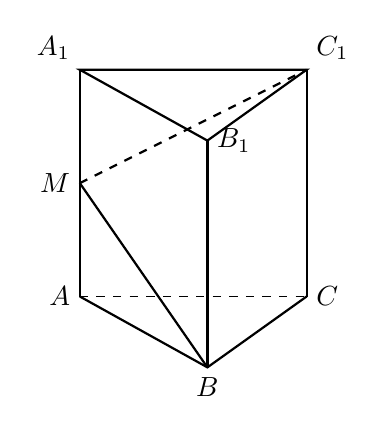
\begin{tikzpicture}[>=stealth, scale=0.9]
  % 顶点坐标
  \coordinate (A) at (0, 0);
  \coordinate (B) at (1.8, -1.0);
  \coordinate (C) at (3.2, 0);
  \coordinate (A1) at (0, 3.2);
  \coordinate (B1) at (1.8, 2.2);
  \coordinate (C1) at (3.2, 3.2);

  % AA1 上的交点 M
  \coordinate (M) at (0, 1.6);

  % 虚线（底面后边 AC 与后侧连线 MC1）
  \draw[dashed, thin] (A) -- (C);
  \draw[dashed, thick] (M) -- (C1);

  % 可见实线（棱与面）
  \draw[thick] (A) -- (B) -- (C);
  \draw[thick] (A1) -- (B1) -- (C1) -- cycle;
  \draw[thick] (A) -- (A1);
  \draw[thick] (B) -- (B1);
  \draw[thick] (C) -- (C1);

  % 折线路径的前半段 BM
  \draw[thick] (B) -- (M);

  % 顶点标签
  \node[left] at (A) {$A$};
  \node[below] at (B) {$B$};
  \node[right] at (C) {$C$};
  \node[left] at (M) {$M$};
  \node[above left] at (A1) {$A_1$};
  \node[right] at (B1) {$B_1$};
  \node[above right] at (C1) {$C_1$};
\end{tikzpicture}
\end{center}
\nopagebreak[4]
\Needspace{0.4\textheight}
\end{question}
\begin{question}
\gkti{17}\textbf{（本小题满分 14 分）} 
如图，抛物线关于 $x$ 轴对称，它的顶点在坐标原点，点 $P(1, 2)$，$A(x_1, y_1)$，$B(x_2, y_2)$ 均在抛物线上．

（1）写出该抛物线的方程及其准线方程；

（2）当 $PA$ 与 $PB$ 的斜率存在且倾斜角互补时，求 $y_1+y_2$ 的值及直线 $AB$ 的斜率．
\nopagebreak[4]
\begin{center}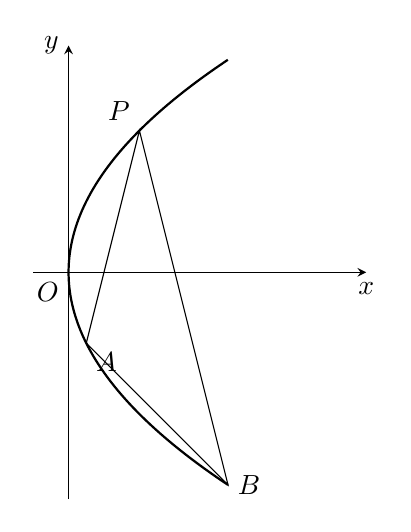
\begin{tikzpicture}[>=stealth, scale=0.9]
  % 坐标轴
  \draw[->] (-0.5, 0) -- (4.2, 0) node[below] {$x$};
  \draw[->] (0, -3.2) -- (0, 3.2) node[left] {$y$};
  \node[below left] at (0, 0) {$O$};

  % 抛物线 y^2 = 4x (x = y^2 / 4)
  \draw[thick, domain=-3.0:3.0, samples=100] plot ({0.25*\x*\x}, {\x});

  % 关键点坐标 (x = y^2/4)
  % P(1, 2)
  \coordinate (P) at (1.0, 2.0);
  % A(0.25, -1.0)
  \coordinate (A) at (0.25, -1.0);
  % B(2.25, -3.0)
  \coordinate (B) at (2.25, -3.0);

  % 连线构成三角形 PAB
  \draw[thin] (P) -- (A) -- (B) -- cycle;

  % 点标注
  \node[above left] at (P) {$P$};
  \node[below right] at (A) {$A$};
  \node[right] at (B) {$B$};
\end{tikzpicture}
\end{center}
\nopagebreak[4]
\end{question}
\begin{question}
\gkti{18}\textbf{（本小题满分 14 分）} 
函数 $f(x)$ 是定义在 $[0, 1]$ 上的增函数，满足 $f(x)=2f\left(\dfrac{x}{2}\right)$ 且 $f(1)=1$，在每个区间 $\left(\dfrac{1}{2^i}, \dfrac{1}{2^{i-1}}\right]$（$i=1, 2, \cdots$）上，$y=f(x)$ 的图象都是斜率为同一常数 $k$ 的直线的一部分．

（1）求 $f(0)$ 及 $f\left(\dfrac{1}{2}\right), f\left(\dfrac{1}{4}\right)$ 的值，并归纳出 $f\left(\dfrac{1}{2^i}\right)$（$i=1, 2, \cdots$）的表达式；

（2）设直线 $x=\dfrac{1}{2^i}$，$x=\dfrac{1}{2^{i-1}}$，$x$ 轴及 $y=f(x)$ 的图象围成的矩形的面积为 $a_i$（$i=1, 2, \cdots$），求 $a_1, a_2$ 及 $\lim_{n\to\infty}(a_1+a_2+\cdots+a_n)$ 的值．

\end{question}
\begin{question}
\gkti{19}\textbf{（本小题满分 12 分）} 
某段城铁线路上依次有 $A, B, C$ 三站，$AB=15\text{ km}$，$BC=3\text{ km}$，在列车运行时刻表上，规定列车 $8$ 时整从 $A$ 站发车，$8$ 时 $07$ 分到达 $B$ 站并停车 $1$ 分钟，$8$ 时 $12$ 分到达 $C$ 站，在实际运行中，假设列车从 $A$ 站正点发车，在 $B$ 站停留 $1$ 分钟，并在行驶时以同一速度 $v\text{ km/h}$ 匀速行驶，列车从 $A$ 站到达某站的时间与时刻表上相应时间之差的绝对值称为列车在该站的运行误差．

（1）分别写出列车在 $B$、$C$ 两站的运行误差；

（2）若要求列车在 $B$、$C$ 两站的运行误差之和不超过 $2$ 分钟，求 $v$ 的取值范围．

\end{question}
\begin{question}
\gkti{20}\textbf{（本小题满分 14 分）} 
给定有限个正数满足条件 $T$：每个数都不大于 $50$ 且总和 $L=1275$．现将这些数按下列要求进行分组，每组数之和不大于 $150$ 且分组的步骤是：

首先，从这些数中选择这样一些数构成第一组，使得 $150$ 与这组数之和的差 $r_1$ 与所有可能的其他选择相比是最小的，$r_1$ 称为第一组余差；

然后，在去掉已选入第一组的数后，对余下的数按第一组的选择方式构成第二组，这时的余差为 $r_2$；如此继续构成第三组（余差为 $r_3$）、第四组（余差为 $r_4$）、$\cdots$，直至第 $N$ 组（余差为 $r_N$）把这些数全部分完为止．

（1）判断 $r_1, r_2, \cdots, r_N$ 的大小关系，并指出除第 $N$ 组外的每组至少含有几个数；

（2）当构成第 $n$（$n<N$）组后，指出余下的每个数与 $r_n$ 的大小关系，并证明 $r_{n-1}>\dfrac{150n-L}{n-1}$；

（3）对任何满足条件 $T$ 的有限个正数，证明：$N\le 11$．

\end{question}